%=====================================================================
\chapter{Research Methodology and Proposed System Implementation}
%=====================================================================

This chapter develops the methodology objective by objective. For each objective it
states the design, describes the implementation as an ordered engineering procedure,
presents the experimental evidence, summarises what was established, and records the
publication in which the work was validated. Section~5.6 then demonstrates how the four
components compose into a single system.

\section{Overall Research Framework and Workflow}

The framework is organised as four layers, shown in Figure~\ref{fig:frame}. Each layer
consumes the output of the previous one and each corresponds to one research objective,
so that a defect in any layer can be located rather than absorbed into an aggregate
performance figure.

\begin{figure}[!htb]
\centering
\scalebox{0.86}{\begin{tikzpicture}[node distance=3mm]
% ---------------- acquisition
\node[blk,minimum width=24mm] (s1) {NSE / BSE\\price and volume};
\node[blk,right=3mm of s1,minimum width=24mm] (s2) {Financial press\\news articles};
\node[blk,right=3mm of s2,minimum width=24mm] (s3) {Social media\\X, StockTwits};
\node[blk,right=3mm of s3,minimum width=24mm] (s4) {RBI, MOSPI\\macro series};
\node[grp,fit=(s1)(s2)(s3)(s4)] (acq) {};
\node[lbl,above=0.5mm of acq] {\textbf{Layer 0 --- data acquisition and temporal alignment}};

% ---------------- layer 1
\node[blkg,below=9mm of s1,minimum width=24mm] (f1) {Technical\\indicator encoder};
\node[blkg,right=3mm of f1,minimum width=24mm] (f2) {Transformer\\news encoder};
\node[blkg,right=3mm of f2,minimum width=24mm] (f3) {Lexicon + RNN\\social encoder};
\node[blkg,right=3mm of f3,minimum width=24mm] (f4) {Engineered\\macro features};
\node[blkg,below=5mm of f2,minimum width=54mm,xshift=13.5mm] (fus)
  {Cross-modal attention and uncertainty-weighted fusion};
\node[grp,fit=(f1)(f2)(f3)(f4)(fus)] (l1) {};
\node[lbl,right=1mm of l1.east,rotate=90,anchor=south,align=center] {\textbf{RO1}};

% ---------------- layer 2
\node[blka,below=8mm of fus,minimum width=54mm] (pred)
  {Optimised deep architecture: Bi-LSTM with attention\\
   and gradient-boosted hybrid predictor};
\node[grp,fit=(pred)] (l2) {};
\node[lbl,right=1mm of l2.east,rotate=90,anchor=south,align=center] {\textbf{RO2}};

% ---------------- layer 3
\node[blk,below=7mm of pred,minimum width=26mm,xshift=-14mm] (cau)
  {Directed causal\\structure};
\node[blk,right=2mm of cau,minimum width=26mm] (dyn)
  {Sentiment noise and\\lead--lag diagnostics};
\node[grp,fit=(cau)(dyn)] (l3) {};
\node[lbl,right=1mm of l3.east,rotate=90,anchor=south,align=center] {\textbf{RO3}};

% ---------------- layer 4
\node[blkg,below=7mm of dyn,minimum width=26mm,xshift=-14mm] (regime)
  {Regime detection\\and risk budget};
\node[blkg,right=2mm of regime,minimum width=26mm] (opt)
  {Constrained portfolio\\optimisation};
\node[grp,fit=(regime)(opt)] (l4) {};
\node[lbl,right=1mm of l4.east,rotate=90,anchor=south,align=center] {\textbf{RO4}};

\node[blkd,below=6mm of opt,minimum width=54mm,xshift=-14mm] (out)
  {Executable allocation, ablated and validated\\ in sample, on holdout and across markets};

\draw[ar] (acq) -- (l1);
\draw[ar] (fus) -- (pred);
\draw[ar] (l2) -- (l3);
\draw[ar] (l3) -- (l4);
\draw[ar] (l4) -- (out);
\draw[arb] (l3.west) to[out=180,in=180] node[lbl,left=1mm,align=right]
  {feedback:\\reliability\\revision} (fus.west);
\end{tikzpicture}}
\caption[Overall research framework]{Overall research framework. Each layer corresponds to one research objective;
the dashed path returns transparency diagnostics to the fusion layer so that a source
found to be noisy is down-weighted rather than merely reported.}
\label{fig:frame}
\end{figure}

The corresponding research workflow is given in Figure~\ref{fig:workflow} as an ordered
sequence of engineering activities. The sequence was executed once end to end and then
revisited iteratively as each objective produced evidence that constrained the next.

\begin{figure}[!htb]
\centering
\scalebox{0.94}{\begin{tikzpicture}[node distance=4mm]
\node[blkd,minimum width=35mm,minimum height=12mm] (w1)
  {\textbf{1. Analyse}\\literature on fusion, sentiment,\\explainability and allocation;\\identify five research gaps};
\node[blk,right=of w1,minimum width=35mm,minimum height=12mm] (w2)
  {\textbf{2. Acquire and align}\\four heterogeneous streams\\to a common trading calendar\\without look-ahead};
\node[blk,right=of w2,minimum width=35mm,minimum height=12mm] (w3)
  {\textbf{3. Engineer}\\technical, textual, social and\\macroeconomic feature\\representations};

\node[blkg,below=of w1,minimum width=35mm,minimum height=12mm] (w4)
  {\textbf{4. Design and develop}\\the fusion network and the\\uncertainty-weighted rule\\\textbf{(RO1)}};
\node[blkg,below=of w2,minimum width=35mm,minimum height=12mm] (w5)
  {\textbf{5. Implement}\\the LLM sentiment pipeline\\and hybrid predictor; optimise\\the architecture \textbf{(RO2)}};
\node[blka,below=of w3,minimum width=35mm,minimum height=12mm] (w6)
  {\textbf{6. Investigate}\\causal structure, sentiment\\noise and sentiment--price\\temporal dynamics \textbf{(RO3)}};

\node[blka,below=of w4,minimum width=35mm,minimum height=12mm] (w7)
  {\textbf{7. Convert}\\the validated signal into an\\allocation under risk, cost and\\turnover constraints \textbf{(RO4)}};
\node[blk,below=of w5,minimum width=35mm,minimum height=12mm] (w8)
  {\textbf{8. Evaluate}\\walk-forward testing,\\specification sweep, ablation\\at matched exposure, holdout};
\node[blkd,below=of w6,minimum width=35mm,minimum height=12mm] (w9)
  {\textbf{9. Validate and compare}\\across sectors, market states\\and a second market; report\\every specification};

\draw[ar] (w1)--(w2); \draw[ar] (w2)--(w3);
\draw[ar] (w3.east) -- ++(3mm,0) |- ($(w3.south)!0.5!(w6.north)$) -| ([xshift=-3mm]w1.west) |- (w4.west);
\draw[ar] (w4)--(w5); \draw[ar] (w5)--(w6);
\draw[ar] (w6.east) -- ++(3mm,0) |- ($(w6.south)!0.5!(w9.north)$) -| ([xshift=-3mm]w4.west) |- (w7.west);
\draw[ar] (w7)--(w8); \draw[ar] (w8)--(w9);
\draw[arb] (w9.east) -- ++(5mm,0) |- node[lbl,pos=0.22,right=1mm] {iterate} (w4.east);
\end{tikzpicture}}
\caption[Research workflow]{Research workflow, read left to right and row by row. The
dashed return path denotes the iteration by which evaluation evidence was used to revise
the fusion and allocation design.}
\label{fig:workflow}
\end{figure}

Table~\ref{tab:data} consolidates the data used across the four objectives. Two
deliberate design decisions are visible in it. First, the study universes differ by
objective because the objectives ask different questions: sectoral breadth is required to
test fusion, single-name depth is required to test sentiment, and cross-asset volatility
dispersion is required to test allocation. Second, the evaluation window lengthens as the
objectives progress, from a ten-year sectoral study to an eighteen-year multi-asset study
with a dedicated holdout, because claims about behaviour under market stress require
observations of market stress.

\begin{table}[!htb]
\centering
\caption[Data sources, universes and evaluation protocols]{Data sources, study universes and evaluation protocols used across the four
research objectives}
\label{tab:data}
\tabfont
\begin{tabular}{@{}L{1.1cm}L{3.3cm}L{3.0cm}L{2.5cm}L{4.2cm}@{}}
\toprule
\textbf{Obj.} & \textbf{Data sources} & \textbf{Universe} & \textbf{Period} &
\textbf{Evaluation protocol} \\
\midrule
RO1 & NSE/BSE prices and 15 technical indicators; financial press; X and StockTwits;
RBI, MOSPI and IMF macro series & NIFTY 50 and ten sectoral indices & Jan 2015 --
Dec 2024 & Chronological 70/15/15 split; training-set-only standardisation; five-fold
expanding-window walk-forward \\
RO2 & Daily OHLCV via \texttt{yfinance}; financial news headlines via news feeds;
transformer sentiment scores & Indian large-capitalisation equities (TCS, RELIANCE,
HDFCBANK) & Multi-year daily & Temporal cross-validation, 80/20 chronological split;
Diebold--Mariano comparison; simulated trading \\
RO3 & Daily and intraday OHLCV; derived multi-granularity features & Five NIFTY50
constituents across five sectors & Jan 2024 -- Mar 2025 (308 sessions) & Conditional
independence testing; backtest against buy-and-hold; budget-window volatility analysis \\
RO4 & Adjusted daily OHLCV; four external published sentiment and stress series used
only for validation & Ten multi-asset ETFs (primary); ten mega-capitalisation equities
(secondary) & Jan 2008 -- Aug 2026 (4{,}689 sessions) & 21-session walk-forward with
10\,bp costs; 18-cell specification sweep; matched-exposure ablation; 665-session
holdout \\
\bottomrule
\end{tabular}
\end{table}

%---------------------------------------------------------------------
\section{Proposed Methodology for Research Objective 1}

\textbf{Research Objective 1:} \emph{To investigate and develop a comprehensive model
that integrates diverse data sources --- such as financial metrics, news articles, social
media sentiment and macroeconomic factors --- aiming to enhance the accuracy of stock
market predictions by providing a holistic analysis.}

\subsection{Design and implementation of the multi-source fusion network}

The Multi-Source Fusion Network is a hierarchical architecture that learns
modality-specific representations before learning cross-modal ones, so that each stream is
encoded in a form appropriate to its own structure. Its layered organisation is shown in
Figure~\ref{fig:msfn}. The implementation proceeds in six steps.

\begin{figure}[!htb]
\centering
\scalebox{0.86}{\begin{tikzpicture}[node distance=3mm]
\node[blkd,minimum width=25mm,minimum height=8mm] (d1) {Financial data\\NSE / BSE};
\node[blkd,right=3mm of d1,minimum width=25mm,minimum height=8mm] (d2) {News articles\\financial press};
\node[blkd,right=3mm of d2,minimum width=25mm,minimum height=8mm] (d3) {Social media\\X, StockTwits};
\node[blkd,right=3mm of d3,minimum width=25mm,minimum height=8mm] (d4) {Macro data\\RBI, MOSPI};

\node[blk,below=6mm of d1,minimum width=25mm,minimum height=8mm] (p1) {15 technical\\indicators};
\node[blk,below=6mm of d2,minimum width=25mm,minimum height=8mm] (p2) {Transformer\\sentiment scoring};
\node[blk,below=6mm of d3,minimum width=25mm,minimum height=8mm] (p3) {Lexicon + LSTM\\sentiment scoring};
\node[blk,below=6mm of d4,minimum width=25mm,minimum height=8mm] (p4) {Normalisation and\\daily interpolation};

\node[blkg,below=6mm of p1,minimum width=25mm,minimum height=8mm] (e1) {CNN\\feature maps};
\node[blkg,below=6mm of p2,minimum width=25mm,minimum height=8mm] (e2) {Text\\embeddings};
\node[blkg,below=6mm of p3,minimum width=25mm,minimum height=8mm] (e3) {Text\\embeddings};
\node[blkg,below=6mm of p4,minimum width=25mm,minimum height=8mm] (e4) {Temporal\\features};

\node[blka,below=7mm of e2,minimum width=79mm,minimum height=8mm,xshift=14mm] (att)
  {Cross-modal attention $\;\to\;$ concatenation $\;\to\;$ adaptive weighting};
\node[blka,below=5mm of att,minimum width=79mm,minimum height=8mm] (bl)
  {Bi-LSTM encoder with temporal attention $\;\to\;$ dense layers with dropout};
\node[blkd,below=5mm of bl,minimum width=79mm,minimum height=7mm] (o)
  {Predicted level and direction with confidence interval, horizon $\tau \in \{1,3,7,15\}$ days};

\foreach \a/\b in {d1/p1,d2/p2,d3/p3,d4/p4,p1/e1,p2/e2,p3/e3,p4/e4}
  \draw[ar] (\a) -- (\b);
\foreach \a in {e1,e2,e3,e4} \draw[ar] (\a.south) -- ++(0,-2mm) -| (att.north);
\draw[ar] (att) -- (bl);
\draw[ar] (bl) -- (o);
\node[lbl,rotate=90,anchor=center,align=center]
  at ([xshift=-7mm]$(d1.west)!0.5!(e1.west)$)
  {acquisition, preprocessing\\and feature extraction};
\node[lbl,rotate=90,anchor=center] at ([xshift=-7mm]d1.west |- att) {fusion};
\node[lbl,rotate=90,anchor=center] at ([xshift=-7mm]d1.west |- o) {output};
\end{tikzpicture}}
\caption[Architecture of the Multi-Source Fusion Network]{Architecture of the Multi-Source Fusion Network, showing the flow from
heterogeneous acquisition through modality-specific preprocessing and feature extraction
to cross-modal fusion and prediction.}
\label{fig:msfn}
\end{figure}

\begin{enumerate}[label=\textbf{Step \arabic*.},leftmargin=4.2em]
\item \textbf{Acquire and align.} Collect price and volume records, news articles, social
media posts and macroeconomic releases, and align every stream to the trading calendar.
Monthly and quarterly macroeconomic series are interpolated to daily frequency; the
consequence --- an understatement of discontinuous announcement-day effects --- is stated
explicitly rather than left implicit.

\item \textbf{Engineer modality features.} Derive fifteen technical indicators covering
trend, momentum, volatility and volume. Score news articles with a domain-adapted
transformer encoder, weighted by relevance and source authority; score social media posts
with a hybrid lexicon and fine-tuned recurrent classifier, retaining daily polarity,
mention volume and sentiment dispersion; normalise the macroeconomic series.

\item \textbf{Encode each modality.} Apply one-dimensional convolutional layers to each
modality $m$, with $h_m^{(l)}$ the representation at layer $l$ and $W_m^{(l)}$,
$b_m^{(l)}$ learnable:
\begin{equation}
h_m^{(l)} = \mathrm{ReLU}\!\left(\mathrm{Conv1D}\!\left(W_m^{(l)} * h_m^{(l-1)} +
b_m^{(l)}\right)\right).
\end{equation}

\item \textbf{Fuse by cross-modal attention.} Compute a relevance weight $\alpha_m =
\mathrm{softmax}(q \cdot k_m / \sqrt{d_k})$ for each modality, where $q$ is a learned
query vector, $k_m$ the key vector of modality $m$ and $d_k$ the key dimension. The
weights are recomputed at each time step, which is what allows source importance to move
with the market state.

\item \textbf{Model temporal dependence.} Pass the fused representation $F_t$ through
bidirectional recurrent layers, $h_t = [\overrightarrow{h}_t ; \overleftarrow{h}_t]$ with
$\overrightarrow{h}_t = \mathrm{LSTM}(F_t, \overrightarrow{h}_{t-1})$ and
$\overleftarrow{h}_t = \mathrm{LSTM}(F_t, \overleftarrow{h}_{t+1})$, and produce the
forecast through dense layers with dropout.

\item \textbf{Evaluate without leakage.} Partition chronologically into training
(2015--2021), validation (2022 -- mid-2023) and test (mid-2023 -- 2024) blocks, standardise
using training-set statistics only, tune hyperparameters on the validation block alone,
and fix random seeds so that reported differences reflect architecture rather than
initialisation.
\end{enumerate}

\subsection{Results and discussion for Research Objective 1}

Table~\ref{tab:msfn} reports the comparison against six baselines together with the source
ablation, presented as a single table because the two questions --- does fusion help, and
which source is responsible --- are answered by the same experiment.

\begin{table}[!htb]
\centering
\caption[Prediction performance and source ablation on the NIFTY 50 index]{One-day-ahead prediction on the NIFTY 50 index: comparison against baselines
(upper block) and source ablation of the proposed model (lower block)}
\label{tab:msfn}
\tabfont
\begin{tabular}{@{}L{4.6cm}L{3.3cm}rrrr@{}}
\toprule
\textbf{Configuration} & \textbf{Data sources} & \textbf{MAE} & \textbf{RMSE} &
\textbf{$R^2$} & \textbf{DA (\%)} \\
\midrule
\multicolumn{6}{@{}l@{}}{\textit{Baseline comparison}}\\
ARIMA & price only & 0.124 & 0.167 & 0.721 & 52.3 \\
LSTM & price only & 0.087 & 0.112 & 0.845 & 61.7 \\
Transformer & price only & 0.079 & 0.103 & 0.869 & 64.2 \\
LSTM + sentiment & price, sentiment & 0.052 & 0.071 & 0.921 & 72.8 \\
LSTM + macro & price, macro & 0.061 & 0.082 & 0.903 & 68.5 \\
Ensemble (simple average) & all, fixed weights & 0.043 & 0.059 & 0.942 & 76.3 \\
\textbf{MSFN (proposed)} & \textbf{all, adaptive fusion} & \textbf{0.018} &
\textbf{0.024} & \textbf{0.988} & \textbf{84.7} \\
\midrule
\multicolumn{6}{@{}l@{}}{\textit{Source ablation of the proposed model}}\\
$-$ financial metrics & news, social, macro & 0.041 & 0.055 & 0.946 & 73.2 \\
$-$ news sentiment & price, social, macro & 0.027 & 0.036 & 0.971 & 79.1 \\
$-$ social media & price, news, macro & 0.025 & 0.033 & 0.976 & 80.8 \\
$-$ macroeconomic & price, news, social & 0.031 & 0.040 & 0.965 & 76.5 \\
$-$ both sentiment sources & price, macro & 0.038 & 0.049 & 0.952 & 74.0 \\
price and technical only & price only & 0.079 & 0.103 & 0.869 & 64.2 \\
\bottomrule
\end{tabular}
\end{table}

Three readings follow. First, adaptive fusion is materially better than fixed-weight
combination: the simple averaging ensemble uses exactly the same four sources and attains
a mean absolute error of 0.043 against 0.018, which isolates the contribution of the
weighting rule rather than of the data. Second, financial metrics remain foundational ---
their removal costs 22.6 per cent of explained variance --- but they are not sufficient,
since restricting the model to price and technical features costs 32.0 percentage points
of directional accuracy. Third, the joint removal of both textual sources costs 10.9 per
cent of explained variance, which exceeds the sum of their individual removals of 5.3 and
3.6 per cent. That superadditivity is the quantitative signature of complementary rather
than redundant information, and it is the empirical justification for a fusion
architecture instead of a larger single-source model.

The learned attention distribution, shown in Figure~\ref{fig:att}, explains where the
gain comes from. Financial metrics carry the highest average weight at 35 per cent, but
that share is not constant: it rises to 42 per cent during earnings season, when
company-specific numerical disclosure dominates, and falls to 28 per cent under high
volatility, when the social media weight rises from 18 to 28 per cent. This is precisely
the behaviour a fixed-weight scheme cannot reproduce, and it is consistent with the
finding that social media sentiment influences Indian sectoral returns most strongly at
market extremes.

\begin{figure}[!htb]
\centering
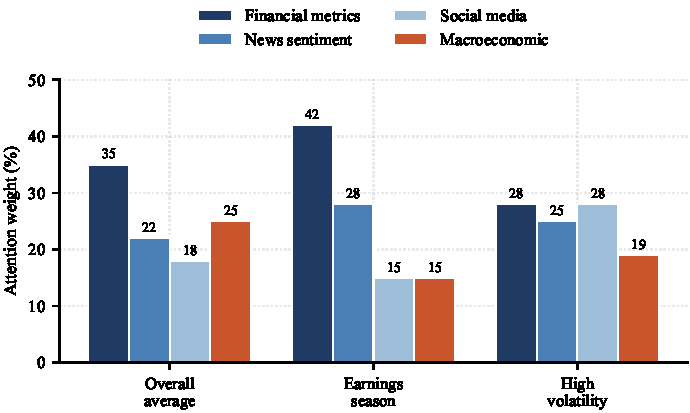
\includegraphics[width=0.80\linewidth]{figs/f_attention.pdf}
\caption[Cross-modal attention weights by market regime]{Cross-modal attention weights learned for each source under three market
regimes. Source importance is state-dependent, which is the property that fixed-weight
fusion cannot represent.}
\label{fig:att}
\end{figure}

Because the headline accuracy is high, the possibility that it is an artefact of a
fortunate split was tested directly. Figure~\ref{fig:wf} shows the expanding-window
protocol and the fold-wise outcome. Normalised errors are tightly clustered at
$0.0016 \pm 0.0004$ and directional accuracy remains above chance in every fold, ranging
from 68 to 92 per cent with a mean of 78.4 per cent. Fold-level $R^2$ averages 0.874,
naturally lower than the full-test value because each short window spans a narrow price
range; the stability of the error magnitudes, not the level of $R^2$, is the relevant
evidence.

\begin{figure}[!htb]
\centering
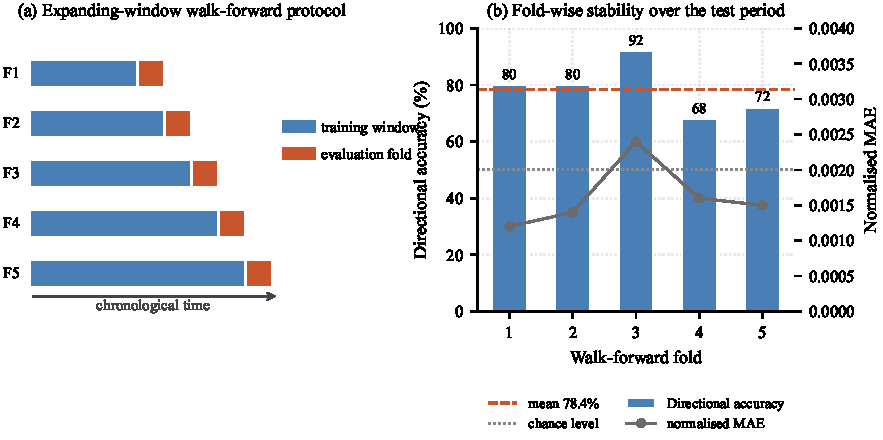
\includegraphics[width=0.99\linewidth]{figs/f_walkforward.pdf}
\caption[Expanding-window walk-forward validation and fold stability]{Expanding-window walk-forward validation. (a) Protocol: each fold is evaluated
only on sessions strictly later than its training window. (b) Fold-wise directional
accuracy and normalised mean absolute error over the test period.}
\label{fig:wf}
\end{figure}

Sector-wise evaluation adds a second dimension. Financials and fast-moving consumer goods
are the most predictable sectors, with $R^2$ above 0.985, while metals and real estate are
the least, below 0.962. The relevant observation is not the ranking but its explanation:
sentiment components contribute most to the globally exposed information technology and
pharmaceutical sectors, whereas energy and metals depend more heavily on macroeconomic
indicators, particularly global commodity prices. Source importance is therefore
structured by sector as well as by regime.

\subsection{Strengthening the fusion rule: dynamic uncertainty weighting}

The attention analysis establishes that source importance varies, but attention weights
are learned once over a training set and express average relevance rather than
instantaneous reliability: a source that has become unreliable in the last two weeks
continues to receive its historical weight. To remove that limitation the fusion rule was
reformulated on a Bayesian basis, shown in Figure~\ref{fig:bayes}.

\begin{figure}[!htb]
\centering
\scalebox{0.86}{\begin{tikzpicture}[node distance=3mm]
\node[blkd,minimum width=27mm,minimum height=8mm] (i1) {Market data\\OHLCV + indicators};
\node[blkd,right=4mm of i1,minimum width=27mm,minimum height=8mm] (i2) {News sentiment\\domain-tuned LLM};
\node[blkd,right=4mm of i2,minimum width=27mm,minimum height=8mm] (i3) {Alternative data\\volatility index};

\node[blk,below=6mm of i1,minimum width=27mm,minimum height=7mm] (m1) {GRU expert $f_M$};
\node[blk,below=6mm of i2,minimum width=27mm,minimum height=7mm] (m2) {Transformer expert $f_S$};
\node[blk,below=6mm of i3,minimum width=27mm,minimum height=7mm] (m3) {MLP expert $f_A$};

\node[blkg,below=6mm of m1,minimum width=27mm,minimum height=7mm] (u1) {$\sigma_{M,t}^2$};
\node[blkg,below=6mm of m2,minimum width=27mm,minimum height=7mm] (u2) {$\sigma_{S,t}^2$};
\node[blkg,below=6mm of m3,minimum width=27mm,minimum height=7mm] (u3) {$\sigma_{A,t}^2$};

\node[blka,below=6mm of u2,minimum width=64mm,minimum height=8mm] (sm)
  {$w_{i,t} = \dfrac{\exp(-\sigma_{i,t}^2 / T)}{\sum_j \exp(-\sigma_{j,t}^2 / T)}$};
\node[blkd,below=5mm of sm,minimum width=64mm,minimum height=7mm] (y)
  {$\hat{y}_t = \sum_i w_{i,t}\, \hat{y}_{i,t}$ \quad --- uncertainty-weighted forecast};

\foreach \a/\b in {i1/m1,i2/m2,i3/m3,m1/u1,m2/u2,m3/u3} \draw[ar] (\a) -- (\b);
\foreach \a in {u1,u2,u3} \draw[ar] (\a.south) -- ++(0,-2mm) -| (sm.north);
\draw[ar] (sm) -- (y);
\draw[arb] (y.east) -- ++(9mm,0) |- node[lbl,right=6mm,align=left,pos=0.25]
  {rolling error\\variance over\\$\tau=10$ sessions} (u3.east);
\node[lbl,rotate=90,anchor=center] at ([xshift=-6mm]m1.west) {expert models};
\node[lbl,rotate=90,anchor=center] at ([xshift=-6mm]u1.west) {uncertainty};
\end{tikzpicture}}
\caption[Bayesian dynamic uncertainty-weighted fusion]{Bayesian dynamic uncertainty-weighted fusion. Each source is discounted in
proportion to the variance of its own recent prediction errors, so reliability is
assessed continuously rather than once at training time.}
\label{fig:bayes}
\end{figure}

The procedure is as follows. \textbf{First}, model each source independently with an
expert network matched to its structure: a gated recurrent unit for the market series, a
transformer encoder for the sentiment sequence, and a multi-layer perceptron for the
volatility index. \textbf{Second}, estimate the predictive uncertainty $\sigma_{i,t}^2$ of
source $i$ as the variance of its prediction errors over a trailing window of
$\tau = 10$ sessions. \textbf{Third}, convert the uncertainties into fusion weights by a
softmax over their negatives, so that a source with a high recent error variance is
automatically down-weighted. \textbf{Fourth}, form the fused prediction as the weighted
sum of expert predictions. \textbf{Fifth}, apply distribution-aware normalisation ---
standard scaling for returns, min--max for sentiment, robust scaling for the heavy-tailed
volatility index --- fitted on an expanding window so that no future information enters
the scaler.

The mechanism self-corrects in a way a static scheme cannot. If a sentiment score is
distorted by an ambiguous or ironic headline and the subsequent market move contradicts
it, the error enters $\sigma_{S,t}^2$ and the sentiment weight falls over the following
sessions without manual intervention. This is the direct methodological answer to gap G1.

The formulation was evaluated on a heterogeneous Nifty~50 dataset spanning January 2018 to
December 2023: index price and volume records with fifteen technical indicators, a daily
sentiment score from a language model fine-tuned on Indian financial news, and the India
VIX as an alternative source of forward-looking volatility. News sentiment is assigned to
the next National Stock Exchange session so that lagged market impact is captured without
look-ahead, market holidays are treated as genuine gaps rather than forward-filled, and
the split is strictly sequential --- 2018--2021 training, 2022 validation, 2023
out-of-sample test --- with the experts pre-trained independently and the system then
fine-tuned end to end through the fusion layer. Table~\ref{tab:bayes} reports the
comparison against the three static fusion strategies identified in Chapter~2.

\begin{table}[!htb]
\centering
\caption[Dynamic uncertainty weighting against static fusion baselines]{Dynamic
uncertainty-weighted fusion against static fusion baselines on the Nifty~50, out-of-sample
year 2023. The source study reports improvements relative to the strongest baseline rather
than absolute levels, so unreported cells are shown as ---.}
\label{tab:bayes}
\tabfont
\begin{tabular}{@{}L{3.1cm}L{5.6cm}L{2.6cm}L{2.9cm}@{}}
\toprule
\textbf{Configuration} & \textbf{Fusion mechanism and source weighting} &
\textbf{Sharpe ratio} & \textbf{Maximum drawdown} \\
\midrule
Early fusion~\cite{moodi2024} & all sources concatenated into one recurrent model;
weights fixed by the architecture & --- & --- \\
Late fusion~\cite{farimani2024} & equal-weight averaging of the three expert
predictions; weights pre-determined & --- & --- \\
Attention fusion~\cite{liu2019attention,haryono2023} & static neural attention over
modalities; weights learned once, then fixed & \textit{strongest baseline} &
\textit{strongest baseline} \\
Proposed architecture, static weights & the same three experts with the uncertainty term
disabled & \multicolumn{2}{L{5.8cm}}{\textit{no better than the baselines above}} \\
\textbf{Proposed dynamic fusion} & softmax over negative predictive uncertainties,
$\tau = 10$ sessions; weights re-estimated every session & \textbf{$+$22.7\%} &
\textbf{$-$18.3\%} \\
\bottomrule
\end{tabular}
\end{table}

Two readings follow. The headline is that against the strongest static competitor the
dynamic rule improves the Sharpe ratio by 22.7 per cent and reduces maximum drawdown by
18.3 per cent, so the gain is in risk-adjusted terms and downside control rather than in
raw accuracy. The second reading matters more here: the ablation row shows that the same
three expert networks, fused with fixed weights, perform no better than the established
baselines. The experts are therefore not the source of the improvement; the weighting rule
is. That isolation is what allows the contribution to be stated precisely as a
fusion-mechanism result rather than an architecture result, and it is the same style of
component-level attribution that Objective~4 later applies to the allocation layer.

The behaviour is also interpretable in the way the design intends. During the volatility
episodes in the test window the weight on the technical expert falls as its recent error
variance rises and migrates to the volatility-index expert and, less strongly, to the
sentiment expert; in calmer trending stretches it returns. Because the shift is driven by
measured error variance rather than by a learned prior, no regime label is required for it
to occur.

\subsection{Summary and validation of Research Objective 1}

The objective is achieved. A four-stream model integrating financial metrics, news
sentiment, social media sentiment and macroeconomic indicators was developed and
evaluated on ten years of Indian market data across ten sectors, attaining a normalised
mean absolute error of 0.018, $R^2$ of 0.988 and directional accuracy of 84.7 per cent
against 76.3 per cent for a fixed-weight ensemble over identical inputs. Ablation
demonstrates that textual sources contribute superadditively, and the attention analysis
that source importance is regime-dependent. The fusion rule was then strengthened from
learned average relevance to measured instantaneous reliability, closing the
static-weighting gap identified in the literature: on the Nifty~50 the dynamic rule
improves the Sharpe ratio by 22.7 per cent and reduces maximum drawdown by 18.3 per cent
against the strongest static-fusion baseline, while the same experts fused with fixed
weights perform no better than that baseline --- which locates the gain in the weighting
mechanism rather than in the networks.

\begin{itemize}
\item \pubcite{P1} --- \emph{A Multi-Source Data Fusion Framework for Enhanced Stock
Market Prediction}, International Conference on Sustainability, Innovation and Technology
(ICSIT), 2026. Supplies the architecture, the ten-sector evaluation, the ablation and the
walk-forward robustness analysis.
\item \pubcite{P4} --- \emph{Dynamic Uncertainty-Weighted Fusion for Multi-Source
Financial Data: A Bayesian Framework for Time-Varying Source Reliability}, communicated to
an international journal. Supplies the uncertainty formulation and the dynamic weighting
mechanism.
\end{itemize}

%---------------------------------------------------------------------
\section{Proposed Methodology for Research Objective 2}

\textbf{Research Objective 2:} \emph{To design a hybrid framework that combines large
language models, sentiment analysis techniques and conventional financial indicators,
focusing on optimising deep learning architectures for real-time stock market
predictions.}

\subsection{Design and implementation of the hybrid LLM--indicator framework}

The framework, shown in Figure~\ref{fig:llm}, is organised as five interconnected layers.
Its design priority is different from that of Objective~1: rather than maximising the
number of sources, it isolates one source --- news text read by a transformer language
model --- and measures precisely what that source adds to a conventional indicator set.

\begin{figure}[!htb]
\centering
\scalebox{0.86}{\begin{tikzpicture}[node distance=3mm]
\node[blkd,minimum width=30mm,minimum height=8mm] (a1) {Historical prices\\OHLCV via API};
\node[blkd,right=8mm of a1,minimum width=30mm,minimum height=8mm] (a2) {Financial news\\headlines and articles};

\node[blk,below=6mm of a1,minimum width=30mm,minimum height=10mm] (b1)
  {\textbf{Technical layer}\\15 indicators: SMA, RSI,\\MACD, Bollinger, VWAP};
\node[blk,below=6mm of a2,minimum width=30mm,minimum height=10mm] (b2)
  {\textbf{Sentiment layer}\\transformer encoder $\rightarrow$\\continuous score $s_t \in [-1,+1]$};

\node[blkg,below=6mm of b1,minimum width=30mm,minimum height=8mm] (c1)
  {$z$-score standardisation};
\node[blkg,below=6mm of b2,minimum width=30mm,minimum height=8mm] (c2)
  {min--max scaling and\\session alignment};

\node[blka,below=6mm of c1,minimum width=68mm,minimum height=8mm,xshift=19mm] (d)
  {\textbf{Feature fusion layer} --- early, feature-level concatenation};
\node[blka,below=5mm of d,minimum width=68mm,minimum height=8mm] (e)
  {\textbf{Model layer} --- gradient-boosted ensemble on the fused space};
\node[blkd,below=5mm of e,minimum width=68mm,minimum height=9mm] (f)
  {\textbf{Evaluation layer} --- temporal cross-validation, directional accuracy,\\
   Diebold--Mariano testing, simulated trading};

\foreach \a/\b in {a1/b1,a2/b2,b1/c1,b2/c2} \draw[ar] (\a) -- (\b);
\draw[ar] (c1.south) -- ++(0,-2mm) -| (d.north);
\draw[ar] (c2.south) -- ++(0,-2mm) -| (d.north);
\draw[ar] (d) -- (e);
\draw[ar] (e) -- (f);
\node[lbl,right=2mm of b2,align=left,xshift=2mm] {contextual reading\\replaces lexicon\\polarity};
\end{tikzpicture}}
\caption[Hybrid language model and technical indicator framework]{Hybrid framework combining large-language-model sentiment extraction with
conventional financial indicators. The continuous sentiment score preserves intensity
that categorical classification would discard.}
\label{fig:llm}
\end{figure}

\begin{enumerate}[label=\textbf{Step \arabic*.},leftmargin=4.2em]
\item \textbf{Collect and synchronise.} Retrieve daily price and volume records for the
target equities and harvest financial news headlines, filtering non-financial content and
prioritising credible sources. Synchronise publication timestamps with session times, so
that news released after the close is attributed to the next trading day.

\item \textbf{Compute technical features.} Derive fifteen indicators covering trend
(moving averages over 5, 10 and 20 sessions), momentum (relative strength index, moving
average convergence divergence with signal line), volatility (Bollinger band measures,
historical volatility) and participation (volume-weighted average price derivatives,
volume momentum).

\item \textbf{Extract sentiment with a language model.} Apply a transformer sentiment
encoder to each headline, retaining a continuous polarity score rather than a class label
together with a confidence score, and batch the inference so that the pipeline remains
tractable in a constrained computational environment.

\item \textbf{Fuse at feature level.} Standardise technical indicators by $z$-score to
equalise scales across measurement units, min--max scale sentiment to preserve its
interpretable range, and concatenate into a single input vector.

\item \textbf{Train and compare.} Train a gradient-boosted tree ensemble on the fused
space~\cite{chen2016xgboost}, chosen for its tolerance of heterogeneous features and
nonlinear interactions, alongside Random Forest, Support Vector Machine and Logistic
Regression baselines on technical indicators alone, so that the incremental value of
sentiment is measured against a like protocol.

\item \textbf{Evaluate honestly.} Partition chronologically at 80/20, apply temporal
cross-validation, test performance differences by Diebold--Mariano statistics, and convert
predictive accuracy into economic terms through a simulated trading strategy.
\end{enumerate}

\subsection{Results and discussion for Research Objective 2}

Table~\ref{tab:llmres} and Figure~\ref{fig:llmres} report the comparison. The result must
be read carefully, because the headline number and the useful number are not the same.

\begin{table}[!htb]
\centering
\caption[Directional classification with LLM-extracted sentiment]{Single-name directional classification with and without LLM-extracted sentiment
features}
\label{tab:llmres}
\tabfont
\begin{tabular}{@{}L{4.6cm}L{3.4cm}rrrr@{}}
\toprule
\textbf{Model} & \textbf{Feature set} & \textbf{Accuracy} & \textbf{Precision} &
\textbf{Recall} & \textbf{F1} \\
\midrule
Random Forest & technical only & 0.4982 & 0.4345 & 0.6033 & 0.5052 \\
Support Vector Machine & technical only & 0.4246 & 0.4246 & 1.0000 & 0.5961 \\
Logistic Regression & technical only & 0.4702 & 0.4257 & 0.7107 & 0.5325 \\
XGBoost with sentiment & technical + LLM sentiment & 0.4772 & 0.4103 & 0.5289 & 0.4621 \\
\midrule
\multicolumn{2}{@{}l}{Mean of technical-only baselines} & 0.4643 & --- & --- & --- \\
\multicolumn{2}{@{}l}{Improvement of the proposed model} & \textbf{+2.77\%} & --- & --- &
--- \\
\bottomrule
\end{tabular}
\end{table}

\begin{figure}[!htb]
\centering
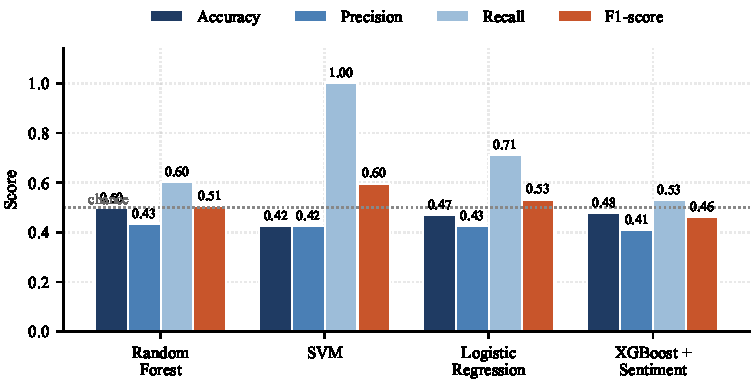
\includegraphics[width=0.90\linewidth]{figs/f_models.pdf}
\caption[Comparative classification performance with sentiment features]{Comparative classification performance. All models operate close to the random
classifier at a single-name daily horizon, which is the correct baseline against which the
sentiment increment should be judged.}
\label{fig:llmres}
\end{figure}

The sentiment-augmented model attains 47.72 per cent accuracy against a baseline mean of
46.43 per cent, a relative improvement of 2.77 per cent. It does not attain the highest
raw accuracy: Random Forest reaches 49.82 per cent. Reporting only the first of these
numbers would misrepresent the finding, so both are stated. What makes the result
meaningful is the structure beneath the aggregate.

\textbf{Feature importance.} In the fused model the sentiment score is the highest-gain
predictor, ranking above established technical features such as the twenty-session moving
average and the moving average convergence divergence. Language-model sentiment is
therefore not a marginal addition the model tolerates; it is the feature the model relies
on most.

\textbf{Orthogonality.} The correlation between the sentiment score and price is 0.04,
while its correlation with momentum indicators reaches 0.74. Sentiment aligns with
momentum, as expected if news and price respond to the same events, yet carries
information essentially independent of price level. This orthogonality is the condition
under which fusion can help at all.

\textbf{Asymmetry across sentiment regimes.} Accuracy measured separately under positive,
neutral and negative sentiment is higher under positive sentiment for all models,
consistent with the asymmetric market response to adverse news. The sentiment-augmented
model varies least across regimes --- a stability property rather than an accuracy
property, and the basis of the economic result.

\textbf{Economic significance.} Despite comparable statistical accuracy, the
sentiment-augmented model produces the highest mean prediction confidence and higher
simulated cumulative returns over a thirty-session trading window, with success rates on
buy signals near 72 and 65 per cent against the baselines. The divergence between
statistical and economic performance is itself the finding: a model that is right no more
often, but is right with better-calibrated confidence, produces better decisions.

\textbf{The limit of the result.} Receiver operating characteristic analysis places all
models close to the random classifier line. Language-model sentiment does not overturn
market efficiency at this horizon, and this report does not claim that it does. What the
evidence supports is that sentiment supplies orthogonal information, improves confidence
calibration and improves buy-side decision quality; establishing where that increment is
large enough to act on is the work of Objective~4.

\subsection{Summary and validation of Research Objective 2}

The framework establishes that language-model sentiment is the highest-importance feature
in the fused space, that it is orthogonal to price-based features, and that it improves
prediction confidence and simulated economic performance while delivering only a small
increment in raw directional accuracy. The bounded nature of that increment is reported
rather than concealed, and it motivates the shift of emphasis in Objective~4 from
statistical accuracy to decision quality.

\begin{itemize}
\item \pubcite{P3} --- \emph{Fusing LLM-Extracted News Sentiment and Market Data for
Enhanced Stock Movement Prediction}, Liberte Journal, ISSN 0024-2020, vol.~14, no.~6,
pp.~424--439, 2026 (published).
\item Supporting architectural evidence for the optimised deep learning component is
provided by \pubcite{P1}, whose Bi-LSTM encoder with attention converges in under two
hours on a single consumer-grade accelerator with approximately 2.1 million trainable
parameters and millisecond forward-pass latency, establishing feasibility at a daily
decision horizon.
\end{itemize}

%---------------------------------------------------------------------
\section{Proposed Methodology for Research Objective 3}

\textbf{Research Objective 3:} \emph{To establish and evaluate an explainable artificial
intelligence framework capable of delivering transparent and interpretable predictions in
stock selection, analysing the impact of sentiment data noise and exploring the temporal
dynamics between sentiment shifts and stock price movements.}

\subsection{Design of the causal and multi-granularity framework}

Transparency is pursued here at the level of structure rather than of attribution. A
post-hoc explanation states which inputs a fitted model used; it does not establish that
those inputs are drivers. The Dynamic-Causal Hybrid Framework, shown in
Figure~\ref{fig:dchf}, therefore constrains the model to features with demonstrable
directed influence before any learning takes place.

\begin{figure}[!htb]
\centering
\scalebox{0.86}{\begin{tikzpicture}[node distance=3mm]
\node[blkd,minimum width=95mm,minimum height=7mm] (in)
  {Daily and intraday price series, five NIFTY50 constituents across five sectors};

\node[blk,below=6mm of in,minimum width=95mm,minimum height=11mm] (s1)
  {\textbf{Stage 1 --- causal graph discovery}\\
   conditional independence testing over lagged series $\Rightarrow$
   time-varying adjacency matrix $A(t)$;\\
   edge $e_{ij}$ retained when $X_i$ improves the prediction of $X_j$ beyond $X_j$'s own past};

\node[blkg,below=5mm of s1,minimum width=95mm,minimum height=12mm] (s2)
  {\textbf{Stage 2 --- multi-scale temporal memory encoding}\\
   parallel recurrent encoders at 1-day, 5-day and 21-day granularity with temporal attention;\\
   $h_t = \mathrm{Debias}\big(\mathrm{Conv}_{1\times k}[\,h^{\text{intraday}}_{t-1},
   h^{\text{daily}}_{t-1}, h^{\text{weekly}}_{t-1}\,]\big)$};

\node[blka,below=5mm of s2,minimum width=95mm,minimum height=11mm] (s3)
  {\textbf{Stage 3 --- credibilistic portfolio optimisation}\\
   returns as triangular fuzzy numbers; range directional measure formulation;\\
   $\max_w \; \big(\mathbb{E}[\tilde{R}] - \lambda\,\mathrm{CVaR}_\alpha(\tilde{R})\big)
   \big/ \mathrm{Entropy}(w)$};

\node[blkd,below=5mm of s3,minimum width=95mm,minimum height=7mm] (out)
  {Sparse, causally traceable portfolio with an auditable feature-selection rationale};

\draw[ar] (in)--(s1); \draw[ar] (s1)--(s2); \draw[ar] (s2)--(s3); \draw[ar] (s3)--(out);
\draw[arb] (s1.west) to[out=180,in=180] node[lbl,left=1mm,align=right]
  {graph refit as\\structure shifts} (s3.west);
\end{tikzpicture}}
\caption[Three-stage Dynamic-Causal Hybrid Framework]{Three-stage Dynamic-Causal Hybrid Framework. Causal discovery constrains the
feature set, multi-granularity encoding captures structure at several horizons, and
credibilistic optimisation converts the signal into holdings under epistemic uncertainty.}
\label{fig:dchf}
\end{figure}

\begin{enumerate}[label=\textbf{Step \arabic*.},leftmargin=4.2em]
\item \textbf{Discover directed structure.} Apply conditional independence
testing~\cite{spirtes2000,granger1969} to lagged closing-price series to construct a
time-varying adjacency matrix $A(t)$, retaining a directed edge only where one series
improves the prediction of another beyond that series' own history.
\item \textbf{Encode multiple horizons.} Run parallel recurrent encoders over short
(1-day), medium (5-day) and long (21-day) windows and combine them through a temporal
attention and debiasing layer, so that volatility clustering at one scale does not obscure
momentum at another.
\item \textbf{Represent uncertainty explicitly.} Express expected returns as triangular
fuzzy numbers, admitting vagueness in the market view rather than forcing a point estimate
the data do not support.
\item \textbf{Optimise and attribute.} Solve for weights maximising entropy-normalised
expected return net of conditional value at risk within the range directional measure
feasible set, backtest against a passive benchmark, and attribute the outcome to
identifiable mechanisms rather than to the aggregate.
\end{enumerate}

\subsection{Results: causal structure as an explanation mechanism}

Table~\ref{tab:causal} gives the recovered adjacency matrix over 308 trading sessions from
January 2024 to March 2025.

\begin{table}[!htb]
\centering
\caption[Dynamic causal adjacency matrix]{Dynamic causal adjacency matrix $A(t)$ over five NIFTY50 constituents. Entry
$(i,j)$ is the strength of the directed influence of row $i$ on column $j$.}
\label{tab:causal}
\tabfont
\begin{tabular}{@{}lrrrrr@{}}
\toprule
\textbf{Influencing $\downarrow$ / Influenced $\rightarrow$} & \textbf{HDFCBANK} &
\textbf{NESTLEIND} & \textbf{RELIANCE} & \textbf{TCS} & \textbf{TITAN} \\
\midrule
HDFCBANK  & 1.000 & 0.299 & 0.791 & 0.079 & 0.460 \\
NESTLEIND & 0.072 & 1.000 & 0.356 & 0.130 & 0.006 \\
RELIANCE  & \textbf{0.913} & 0.324 & 1.000 & \textbf{0.650} & \textbf{0.849} \\
TCS       & 0.110 & 0.670 & 0.516 & 1.000 & 0.436 \\
TITAN     & 0.337 & 0.058 & 0.216 & 0.610 & 1.000 \\
\bottomrule
\end{tabular}
\end{table}

The recovered graph has a density of 0.850 and a maximum causal score of 1.000,
indicating strong directed interdependence among the constituents. Its most interpretable
feature is that RELIANCE acts as a systematic causal hub: it exerts strong directed
influence on HDFCBANK (0.913), TITAN (0.849) and TCS (0.650) while receiving markedly
weaker influence in return. Figure~\ref{fig:graph} renders the structure above an edge
threshold of 0.3.

\begin{figure}[!htb]
\centering
\scalebox{0.86}{\begin{tikzpicture}[node distance=20mm,
  nd/.style={circle,draw=black!70,fill=blue!6,minimum size=13mm,font=\scriptsize,align=center},
  hub/.style={circle,draw=black!80,fill=orange!22,minimum size=15mm,font=\scriptsize\bfseries,align=center},
  ce/.style={-{Latex[length=1.6mm,width=1.2mm]},draw=black!60},
  cs/.style={-{Latex[length=1.9mm,width=1.5mm]},draw=black!85,line width=1.0pt}]
\node[hub] (rel) at (0,0) {RELI-\\ANCE};
\node[nd] (hdfc) at (-32mm,14mm) {HDFC\\BANK};
\node[nd] (tcs) at (32mm,14mm) {TCS};
\node[nd] (titan) at (-24mm,-20mm) {TITAN};
\node[nd] (nest) at (26mm,-20mm) {NESTLE\\IND};

\draw[cs] (rel) -- node[lbl,above,sloped,font=\tiny] {0.913} (hdfc);
\draw[cs] (rel) -- node[lbl,above,sloped,font=\tiny] {0.849} (titan);
\draw[cs] (rel) -- node[lbl,above,sloped,font=\tiny] {0.650} (tcs);
\draw[ce] (hdfc) to[bend left=14] node[lbl,above,sloped,font=\tiny] {0.791} (rel);
\draw[ce] (hdfc) to[bend right=28] node[lbl,left,font=\tiny] {0.460} (titan);
\draw[ce] (tcs) to[bend left=18] node[lbl,right,font=\tiny] {0.670} (nest);
\draw[ce] (tcs) to[bend left=10] node[lbl,below,sloped,font=\tiny] {0.516} (rel);
\draw[ce] (titan) to[bend right=16] node[lbl,below,font=\tiny] {0.610} (tcs);
\draw[ce] (nest) to[bend left=12] node[lbl,below,sloped,font=\tiny] {0.356} (rel);
\node[lbl,below=3mm of titan,align=left,xshift=8mm]
  {Graph density 0.850; edges shown for strength $>0.3$.\\
   Bold edges mark the causal hub, whose outgoing\\ influence exceeds its incoming influence.};
\end{tikzpicture}}
\caption[Dynamic causal graph recovered from NIFTY50 constituents]{Dynamic causal graph recovered from NIFTY50 constituent series. The structure is
readable, which is the property that makes the feature selection auditable.}
\label{fig:graph}
\end{figure}

The decisive evidence for the approach is the comparison between correlation and
causality. Pairs exist in this universe --- RELIANCE on TITAN being the clearest --- for
which the directed causal influence is high while the linear correlation is low, and a
correlation-based selector would have discarded that relationship. This is the mechanistic
justification for the framework: transparency and accuracy are not in tension here,
because the causal constraint retains information the correlational alternative destroys.

Performance over the study window is reported in full. The strategy attained a Sharpe
ratio of 0.377 with a win rate of 48.8 per cent, and underperformed buy-and-hold by 8.95
per cent during a strong bull market. A win rate below one half combined with a positive
Sharpe ratio indicates asymmetric profit capture, with winning trades larger than losing
ones; transaction costs and signal lag account for the nominal shortfall. The framework is
therefore a capital-preservation instrument rather than a return-maximising one. Peak
volatility of 77.67 per cent during the 2024 Union Budget window shows the limit of the
debiasing layer, whose stationarity assumption fails exactly when policy shocks change the
noise process --- a diagnostic rather than fatal result, since it identifies
non-stationary debiasing as a specific, addressable weakness.

\subsection{Sentiment noise and sentiment--price temporal dynamics}

The second half of the objective concerns how noisy the sentiment channel is and how
sentiment shifts relate in time to price movements. Three instruments were used.

\textbf{Construct validation against external evidence.} Naming a series a sentiment
measure is a claim testable independently of whether it makes money. The market-derived
composite~\cite{bakerwurgler2007} was compared against four independently published
series, none of which enters the framework at any stage: a household survey of consumer
sentiment, an implied volatility index, a financial stress index and a financial
conditions index. Figure~\ref{fig:sent}(a) reports the outcome. Every correlation carries
the expected sign --- positive against the survey, negative against the three stress and
volatility measures --- and every one is significant in first differences at the five per
cent level. The survey comparison is the informative one, because the two series share no
inputs: a correlation of $+0.240$ between monthly changes in a composite built from
exchange turnover and monthly changes in what households report to an interviewer cannot
be a mechanical artefact of shared construction. The sign is correct in all sixteen
series-by-sub-period combinations, with magnitudes largest in crisis periods, which is the
expected pattern for a stress-sensitive measure.

\begin{figure}[!htb]
\centering
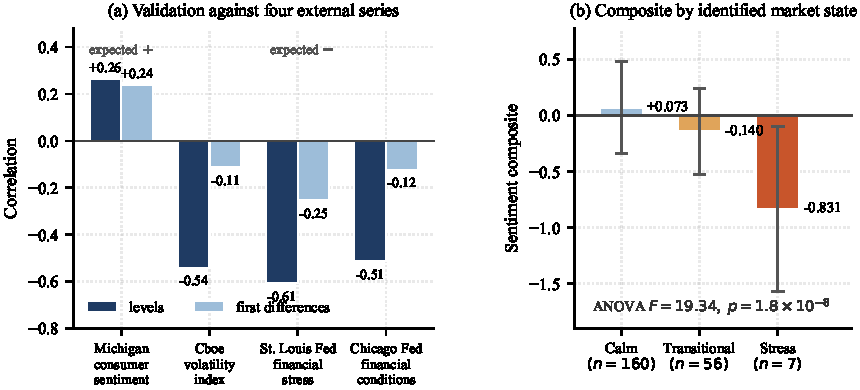
\includegraphics[width=0.99\linewidth]{figs/f_sentiment_diag.pdf}
\caption[Sentiment composite diagnostics]{Sentiment diagnostics. (a) Correlation of the sentiment composite with four
independently published series in levels and first differences. (b) The composite
evaluated by identified market state; the states are labelled by fitted volatility and the
composite plays no part in fitting them.}
\label{fig:sent}
\end{figure}

\textbf{Separation across market states.} If the identified states are states of sentiment
as well as of volatility, the composite should differ across them.
Figure~\ref{fig:sent}(b) shows a monotone and steep ordering: $+0.073$ in the calm state,
$-0.140$ in the transitional state and $-0.831$ in the stress state. One-way analysis of
variance gives $F = 19.34$ with $p = 1.8 \times 10^{-8}$, and the rank-based
Kruskal--Wallis test, safer given only seven observations in the stress state, gives
$H = 29.54$ with $p = 3.9 \times 10^{-7}$. Since the mixture model is fitted on realised
volatility and short-horizon momentum, and the composite is not among its inputs, this
separation on a withheld variable justifies describing the states as
sentiment-and-volatility states rather than volatility states alone.

\textbf{Noise and lead--lag structure.} Two further findings characterise the channel. In
\pubcite{P3}, the temporal overlay of sentiment against price shows that strong sentiment
spikes frequently precede major price changes, but that the mapping from magnitude to
direction is not simple: sustained positive sentiment accompanies gradual advances,
whereas sharp negative spikes accompany abrupt declines. The sentiment distribution is
approximately symmetric about neutral with moderate tails, indicating that the extraction
pipeline captures genuine variation rather than producing a biased categorical output. In
\pubcite{P5}, the predictive content of the validated composite, measured as a
cross-sectional information coefficient, is indistinguishable from zero or significantly
negative depending on the period. Keeping these two results apart is essential: a
composite can measure sentiment accurately and still fail to forecast returns, and
conflating construct validity with predictive usefulness is a common error in this
literature.

\subsection{Summary and validation of Research Objective 3}

Transparency here derives from directed causal structure rather than from post-hoc
attribution alone, and multi-scale temporal encoding makes the horizon of each signal
explicit. The framework recovers an interpretable causal graph of density 0.850 with an
identifiable hub and demonstrates that causal influence and linear correlation can
diverge, which is the justification for causal feature selection. Sentiment noise was
quantified rather than assumed: the construct was validated against four external series
with the correct sign in all sixteen series-by-period combinations and separates market
states at $p = 1.8 \times 10^{-8}$, yet carries no reliable directional information --- a
distinction reported in full because it constrains how sentiment should be used
downstream.

\begin{itemize}
\item \pubcite{P2} --- \emph{A Dynamic-Causal Hybrid Framework for NIFTY50 Stock Decision
Making: A Multi-Granularity Temporal Learning Approach}, international conference
(communicated). Supplies causal discovery, multi-granularity encoding and credibilistic
allocation.
\item \pubcite{P3} and \pubcite{P5} supply the sentiment-noise and temporal-dynamics
evidence, as described above.
\end{itemize}

%---------------------------------------------------------------------
\section{Proposed Methodology for Research Objective 4}

\textbf{Research Objective 4:} \emph{To evaluate and validate the result and practical
application of the proposed model across different stock markets, exploring transfer
learning techniques for cross-market applications and validating the model against
benchmark datasets and real-world market data.}

\subsection{Design of the decision-theoretic allocation framework}

The framework, shown in Figure~\ref{fig:alloc}, converts a fused signal into an
executable portfolio in a way that keeps two decisions separate: what to hold relative to
everything else, and how much total risk to carry. That separation is what makes each
layer independently testable.

\begin{figure}[!htb]
\centering
\scalebox{0.86}{\begin{tikzpicture}[node distance=3mm]
\node[blkd,minimum width=96mm,minimum height=8mm] (f)
  {\textbf{Stage 1 --- causal feature construction:} nine causal features per asset per
   session, cross-sectionally standardised\\ into a technical composite and a sentiment
   composite};

\node[blk,below=5mm of f,minimum width=46mm,minimum height=13mm,xshift=-25mm] (g)
  {\textbf{Stage 2a --- regime identification}\\
   Gaussian mixture, $K=3$, expanding\\ window, components anchored by\\
   ascending fitted volatility:\\ calm / transitional / stress};
\node[blk,right=4mm of g,minimum width=46mm,minimum height=13mm] (h)
  {\textbf{Stage 2b --- signal fusion}\\
   $z_{i,t} = c_{i,t}\big(w^T_{r_t} T_{i,t} + w^M_{r_t} M_{i,t}\big)$\\
   scaled to a return metric by\\ $\alpha_{i,t} = \mathrm{IC}\cdot\sigma_{i,t}\cdot z_{i,t}$};

\node[blkg,below=5mm of g,minimum width=46mm,minimum height=13mm] (qp)
  {\textbf{Stage 3a --- relative composition}\\
   $\max_w \alpha_t^{\!\top} w - \lambda w^{\!\top}\Sigma_t w - \kappa\|w-w_{t-1}\|_1$\\
   s.t. $w\ge 0$, $w \le 0.25$, $\mathbf{1}^{\!\top} w = 1$;\\
   $\Sigma_t$ by Ledoit--Wolf shrinkage};
\node[blkg,right=4mm of qp,minimum width=46mm,minimum height=13mm] (rb)
  {\textbf{Stage 3b --- total risk}\\
   $w_t^{*} = k_{r_t}\,\tilde{w}_t$, with\\
   $k = \{1.00,\,0.75,\,0.50\}$ as a fraction\\ of the sleeve's own volatility};

\node[blka,below=5mm of qp,minimum width=96mm,minimum height=12mm,xshift=25mm] (ev)
  {\textbf{Stage 4 --- evaluation and ablation:} 21-session walk-forward with 10\,bp costs;
   18-cell specification sweep;\\ matched-exposure ablation; four stress episodes;
   665-session holdout; secondary market universe;\\
   Newey--West and stationary block bootstrap inference};

\draw[ar] (f.south) -- ++(0,-2mm) -| (g.north);
\draw[ar] (f.south) -- ++(0,-2mm) -| (h.north);
\draw[ar] (g) -- (qp);
\draw[ar] (h) -- (qp);
\draw[ar] (g.east) -- (h.west);
\draw[ar] (qp) -- (rb);
\draw[ar] (rb.south) -- ++(0,-2mm) -| (ev.north);
\draw[ar] (qp.south) -- ++(0,-2mm) -| (ev.north);
\end{tikzpicture}}
\caption[Decision-theoretic allocation framework]{Decision-theoretic allocation framework. Stage 3 deliberately separates relative
composition from total risk, which is the design property that makes the matched-exposure
ablation of Section~5.5.2 possible.}
\label{fig:alloc}
\end{figure}

The implementation proceeds as follows. \textbf{First}, compute nine causal features per
asset per session and standardise them cross-sectionally, so that a value expresses how an
asset ranks against its peers on that day rather than against its own history; this also
removes the common market factor, preventing a market-wide move from registering as a
signal on every asset at once. \textbf{Second}, identify the market state with a
three-component Gaussian mixture over rolling volatility and rolling momentum, refitted at
every rebalance on an expanding window of strictly earlier sessions, with components
sorted by ascending fitted volatility so that state labels remain comparable across
refits. \textbf{Third}, fuse the two composites with state-dependent weights and a
confidence term that discounts assets whose composites disagree, then place the fused
score on a return scale by information-ratio scaling~\cite{grinold2000}. \textbf{Fourth},
solve the constrained quadratic program for the fully invested risky sleeve, with
covariance shrinkage, a 25 per cent position cap and a turnover penalty annualising a
one-way cost of ten basis points. \textbf{Fifth}, scale the sleeve by the regime risk
budget, holding the residual in cash; scaling is one-sided, so the framework de-risks in
disturbed states but never levers up, and any performance difference is attributable to
risk reduction rather than to leverage.

Two implementation details proved consequential and generalise beyond this framework.
Mixture component indices permute freely between refits, so labels must be anchored;
omitting the anchoring step produces no error, only a silently scrambled regime series.
And the risk budget must be expressed as a fraction of the portfolio's own volatility
rather than as an absolute target, because absolute targets calibrated for concentrated
equity portfolios are never reached by a diversified sleeve and leave the regime layer
present in the specification but inert.

\subsection{Results and discussion for Research Objective 4}

Table~\ref{tab:port} consolidates the evaluation across the primary universe, the
holdout, the specification sweep and the secondary market.

\begin{table}[!htb]
\centering
\caption[Portfolio-level evaluation across universes and periods]{Portfolio-level evaluation. Benchmarks are rebalanced daily and charged no
transaction costs, which is deliberately unfavourable to the proposed framework.}
\label{tab:port}
\tabfont
\begin{tabular}{@{}L{5.5cm}rrrrr@{}}
\toprule
\textbf{Configuration} & \textbf{CAGR} & \textbf{Vol.} & \textbf{Sharpe} &
\textbf{Max DD} & \textbf{Calmar} \\
\midrule
\multicolumn{6}{@{}l@{}}{\textit{Primary universe: ten multi-asset ETFs, Jan 2008 -- Aug
2026, 4{,}689 sessions}}\\
Proposed regime-conditional framework & 5.65\% & 6.44\% & \textbf{0.878} &
\textbf{$-$18.98\%} & 0.298 \\
Equal-weight benchmark & 8.45\% & 13.45\% & 0.628 & $-$36.08\% & 0.234 \\
Inverse-volatility benchmark & 7.46\% & 8.78\% & 0.849 & $-$24.09\% & 0.309 \\
Equal-weight at strategy volatility & 4.19\% & 6.44\% & 0.651 & $-$18.69\% & 0.224 \\
\midrule
\multicolumn{6}{@{}l@{}}{\textit{Out-of-sample holdout: 665 sessions, Jan 2024 -- Aug
2026}}\\
Proposed framework & --- & --- & \textbf{1.614} & \textbf{$-$5.48\%} & --- \\
Equal-weight benchmark & --- & --- & 1.391 & $-$10.13\% & --- \\
Inverse-volatility benchmark & --- & --- & 1.397 & $-$6.70\% & --- \\
Equal-weight at strategy volatility & --- & --- & 1.378 & $-$7.04\% & --- \\
\midrule
\multicolumn{6}{@{}l@{}}{\textit{Specification sweep: 3 seeds $\times$ 2 covariance
windows $\times$ 3 rebalance intervals}}\\
Range across all 18 cells & --- & --- & 0.813 -- 0.956 & $-$21.1\% -- $-$19.0\% & --- \\
Cells beating the benchmark on both measures & \multicolumn{5}{l}{18 of 18} \\
\midrule
\multicolumn{6}{@{}l@{}}{\textit{Secondary universe: ten mega-capitalisation equities,
2019 -- 2026 (cross-market transfer)}}\\
Proposed framework & 17.02\% & 14.87\% & 1.145 & \textbf{$-$20.45\%} & --- \\
Equal-weight benchmark & 33.52\% & 24.45\% & \textbf{1.371} & $-$33.63\% & --- \\
\bottomrule
\end{tabular}
\end{table}

On the primary universe the framework raises the Sharpe ratio from 0.628 to 0.878, a gain
of 40 per cent, and reduces maximum drawdown from $-36.08$ to $-18.98$ per cent, a
reduction of 47 per cent, while earning a lower compound return of 5.65 against 8.45 per
cent per annum. It is a risk-reduction instrument whose return sacrifice is smaller than
its risk reduction, and it is presented as such. Against the volatility-matched benchmark
it retains its Sharpe advantage but loses marginally on drawdown, which bounds the
drawdown claim precisely: the framework reduces drawdown relative to an unlevered
diversified benchmark, not relative to every portfolio held at the same volatility.

The holdout block is the strongest single piece of evidence, because every specification
decision --- universe, feature set, number of regimes, risk budget, rebalancing interval
and cost assumption --- was fixed before any session in it was examined. On those 665
sessions the framework records a higher Sharpe ratio and a smaller drawdown than all three
benchmarks, and two of those comparisons reverse the in-sample ordering. Three
qualifications are stated alongside: 665 sessions cannot settle the question on their own,
the period contains no episode comparable to 2008 or 2020, and the framework again earns
less in absolute terms.

Figure~\ref{fig:abl} isolates where the performance originates.

\begin{figure}[!htb]
\centering
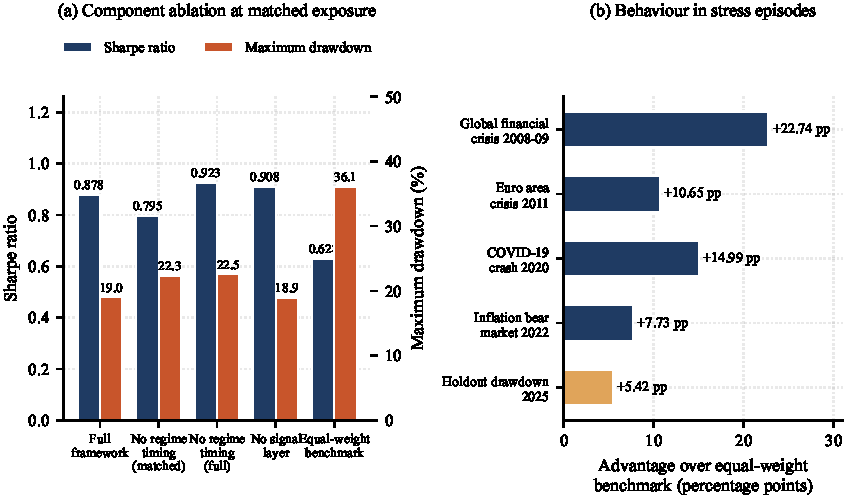
\includegraphics[width=0.99\linewidth]{figs/f_ablation.pdf}
\caption[Component ablation and stress-episode behaviour]{(a) Component ablation. The matched-exposure control carries the same average
invested exposure as the full framework but applies it without regard to the regime, so
that only the timing of risk differs. (b) Cumulative advantage over the benchmark in four
stress episodes chosen on documented market history, plus the deepest benchmark drawdown
in the holdout.}
\label{fig:abl}
\end{figure}

The ablation answers the objective's central question. Holding average exposure fixed at
92.1 per cent, allocating that exposure according to the identified regime rather than
uniformly raises the Sharpe ratio from 0.795 to 0.878 and improves maximum drawdown from
$-22.26$ to $-18.98$ per cent, with no significant difference in mean return
($p = 0.695$). That combination --- both measures improve, mean return does not change ---
is the signature of a genuine risk-timing effect rather than of simply holding less, and
it is available only because the control was constructed at matched risk. The cost of that
timing is also measured: against a fully invested variant the framework gives up
approximately 1.3 percentage points of annual return, significantly so ($p = 0.016$), in
exchange for 3.55 percentage points of maximum drawdown.

The same ablation returns a null on the signal fusion layer. Removing it entirely, so that
the optimiser becomes a constrained minimum-variance problem, moves the Sharpe ratio from
0.878 to 0.908 and maximum drawdown from $-18.98$ to $-18.87$ per cent; both movements
favour removal and neither is significant ($p = 0.650$). The information coefficients
explain why: both composites are significantly negatively related to next-session
cross-sectional returns over the full sample, and the state-dependent weighting hypothesis
--- that sentiment becomes relatively more informative under stress --- is not supported,
with point estimates running the other way and the calm-to-stress contrast insignificant
($t = -1.46$, $p = 0.145$). The negative relationship is not stable enough to exploit by
inversion either: it is $-0.039$ before 2024 and $+0.009$ afterwards.

This null is retained in full rather than removed. Component-level negative results are
rarely published, which is one reason architectures accumulate layers whose contribution
has never been isolated; reporting which layer works is more useful than an aggregate
number that conceals the distinction, and it is why the ablation design of
Figure~\ref{fig:alloc} was built into the framework rather than added afterwards.

Behaviour under stress, in Figure~\ref{fig:abl}(b), is consistent across four episodes
selected before the analysis on documented market history rather than by inspection of
results. The framework outperforms in all four, by between 7.7 and 22.7 percentage points,
and by a further 5.4 points in the deepest benchmark drawdown of the holdout. Its average
return on the worst 5 per cent of benchmark sessions is $-0.59$ per cent against $-2.01$
per cent, a cushion of 1.42 points per session. Downside capture is 0.38 and upside
capture 0.41, a capture ratio of 0.93: the framework participates less in both directions
in roughly equal proportion, so its advantage comes from carrying less risk in adverse
states rather than from directional skill.

On statistical significance the report is equally direct. The Sharpe difference of
$+0.250$ carries a 95 per cent bootstrap interval of $[-0.102, 0.574]$, which includes
zero, and the shortfall in mean return is not significant ($p = 0.171$). Eighteen years of
daily data contain only four independent observations of the events that matter for a
drawdown claim, and no amount of daily sampling converts that into statistical power. What
is robust is consistency, not the point estimate: the Sharpe advantage appears in 18 of 18
specifications, the drawdown advantage in 18 of 18 specifications and 18 of 19 calendar
years, and the outperformance in all four stress episodes. Robustness and significance are
different properties and are not conflated here.

\subsection{Cross-market transfer}

Transfer was tested by running the framework without modification on a second universe of
ten mega-capitalisation United States equities over 2019--2026. The outcome is mixed and
is reported as such. The framework loses on risk-adjusted return, 1.145 against 1.371, and
gives up 15.09 percentage points of annual return, significantly so ($t = -2.791$,
$p = 0.005$). Its defensive behaviour nevertheless survives intact: maximum drawdown
improves from $-33.63$ to $-20.45$ per cent, it wins on drawdown in eight of eight
calendar years, and it outperforms in both stress episodes the window contains, by 12.50
percentage points in the 2020 crash and 12.60 points in the 2022 bear market. Critically,
the regime layer itself continues to behave as designed: against the matched-exposure
control it improves both the Sharpe ratio and the drawdown, so the risk-timing effect
reproduces in a universe where the framework loses overall.

One point of scope should be stated plainly rather than glossed. The objective refers to
\emph{transfer learning} for cross-market application; what has been carried out here is
direct transfer. The framework, its feature definitions and its fitted procedure were
applied to the second universe without modification and without any adaptation step, which
is the stricter test of whether the mechanism itself generalises: no parameter was
fine-tuned on the target market, no representation was pre-trained and re-used, and no
domain-adaptation objective was optimised. The result below is therefore a lower bound on
cross-market performance, and adaptation-based transfer is identified as open work in
Section~7.2 rather than claimed here.

The explanation is a property of the universe rather than of the framework. Ten
mega-capitalisation equities are close to a single factor bet: correlations are high,
there is no low-volatility asset to rotate into, and the risky sleeve carries roughly 15
per cent annualised volatility against 6 per cent in the multi-asset case. De-risking
there can only move capital to cash, so the framework systematically forgoes return during
an exceptional advance. The transferability condition is therefore explicit and testable
in advance: the framework requires a universe with genuine dispersion in asset volatility.
Complementary cross-market evidence at sectoral granularity comes from the ten-sector
evaluation of \pubcite{P1} and the sector-level regime behaviour of \pubcite{P2}.

\subsection{Summary and validation of Research Objective 4}

The framework was evaluated as a decision system rather than as a predictor. It improves
risk-adjusted return and materially reduces drawdown against an unlevered diversified
benchmark, sustains that behaviour on a holdout that postdates every design decision, and
does so consistently across every specification examined. Ablation at matched exposure
locates the gain in regime-conditional risk timing and returns a null on the signal fusion
layer, and cross-market transfer establishes a precise boundary condition for
applicability. The limits of the evidence --- an insignificant Sharpe improvement, few
independent stress events, a lower absolute return --- are stated explicitly.

\begin{itemize}
\item \pubcite{P5} --- \emph{From Signal Fusion to Asset Allocation: A Decision-Theoretic
Model for Portfolio Construction Under Regime-Based Sentiment and Volatility},
\emph{International Journal of Applied Decision Sciences} (Inderscience), manuscript
IJADS-312370, under review. Supplies the framework, the eighteen-year
evaluation, the specification sweep, the ablation, the holdout and the cross-market test.
\item \pubcite{P1} and \pubcite{P2} supply supporting sectoral and regime-level
cross-market evidence.
\end{itemize}

%---------------------------------------------------------------------
\section{Integration of the Individual Contributions}

The four contributions are not four independent studies with a shared subject. Each was
produced in response to a limitation exposed by the one before it, and the composed system
is shown in Figure~\ref{fig:integrated}.

\begin{figure}[!htb]
\centering
\scalebox{0.86}{\begin{tikzpicture}[node distance=3mm]
\node[blkd,minimum width=98mm,minimum height=6.5mm] (i)
  {Heterogeneous inputs: market records, financial news, social media, macroeconomic
   series, volatility indices};

\node[blk,below=5mm of i,minimum width=98mm,minimum height=10mm] (c1)
  {\textbf{RC1 --- integration.} Four-stream fusion with cross-modal attention; source
   weights conditioned on\\ measured, time-varying reliability \hfill
   \textit{establishes: what to fuse, and how much to trust each stream}};

\node[blkg,below=4mm of c1,minimum width=98mm,minimum height=10mm] (c2)
  {\textbf{RC2 --- signal extraction.} Language-model sentiment fused with technical
   indicators in an optimised\\ architecture \hfill
   \textit{establishes: sentiment is the highest-importance feature, and its increment is
   bounded}};

\node[blka,below=4mm of c2,minimum width=98mm,minimum height=10mm] (c3)
  {\textbf{RC3 --- transparency.} Directed causal structure replaces correlation;
   sentiment validated externally\\ and its noise measured \hfill
   \textit{establishes: which relationships are real, and how far sentiment can be
   trusted}};

\node[blkg,below=4mm of c3,minimum width=98mm,minimum height=10mm] (c4)
  {\textbf{RC4 --- decision.} Regime-conditional allocation under cost, turnover and
   position constraints;\\ ablated at matched risk \hfill
   \textit{establishes: which layer produces the outcome, and where it transfers}};

\node[blkd,below=5mm of c4,minimum width=98mm,minimum height=7mm] (o)
  {An integrated framework whose every layer has been separately tested, with its
   applicability bounded by evidence};

\draw[ar] (i) -- (c1); \draw[ar] (c1) -- (c2); \draw[ar] (c2) -- (c3);
\draw[ar] (c3) -- (c4); \draw[ar] (c4) -- (o);
\draw[arb] (c2.east) -- ++(6mm,0) |- node[lbl,right=3mm,pos=0.25,align=left]
  {bounded increment\\$\Rightarrow$ measure noise} (c3.east);
\draw[arb] (c3.west) -- ++(-6mm,0) |- node[lbl,left=3mm,pos=0.25,align=right]
  {validated construct\\$\Rightarrow$ testable claim} (c4.west);
\end{tikzpicture}}
\caption[Integration of the four research contributions]{Integration of the four contributions. Each layer is a response to a limitation
exposed by the previous one, and the dashed paths show the two places where a finding in
one study redirected the design of the next.}
\label{fig:integrated}
\end{figure}

The logic of the progression is as follows. Contribution~1 established that fusing four
sources improves prediction and that the value of each source is state-dependent, which
raised the question of how to weight a source whose reliability changes --- answered by
the uncertainty-weighted formulation. Contribution~2 isolated the language-model sentiment
channel and found it the most important single feature yet delivering only a bounded
increment in raw accuracy, which raised the question of whether the limitation lies in the
measurement or in the horizon. Contribution~3 answered by separating the two: the
sentiment construct was validated externally and found sound, while its predictive content
was measured separately and found weak, so the limitation is not one of measurement.
Contribution~4 followed directly. If the signal channel is bounded, the framework must
earn its value at the decision layer, and the ablation confirms exactly this: risk timing
by market state works, and the signal layer does not. The final system is therefore not
the one originally envisaged, and it is better supported for that reason.
